Modern interactive 3D applications, like video games, VR/AR apps, simulators etc., depend on believable lighting interactions with the objects of a 3D scene to achieve the desired visual goals, while trying to maintain real-time frame-rate budgets, typically above 30 Frames per Second (FPS). Achieving visual fidelity and performance can be a difficult task and sometimes impossible with the given hardware specifications of the device. For that reason, modern real-time rendering engines, e.g. Unity, Unreal Engine, Godot and others, depend on a number of methods to balance those metrics. 

The illumination of any scene can be split into two very simple categories. Direct Illumination, the light that travels unoccluded from a light source to a surface of an object, is typically handled with techniques like shadow-mapping or screen-space shadows, yielding crisp, high-framerate-capable shadows, but lack in inter-surface light transport situations. In contrast, Indirect Illumination, or Global Illumination (GI), captures light that has bounced or refracted off one or more surfaces, producing soft shadows, color bleeding, and contextually rich shading. 

\begin{figure}[!htb]
	\begin{minipage}{0.48\textwidth}
		\centering
		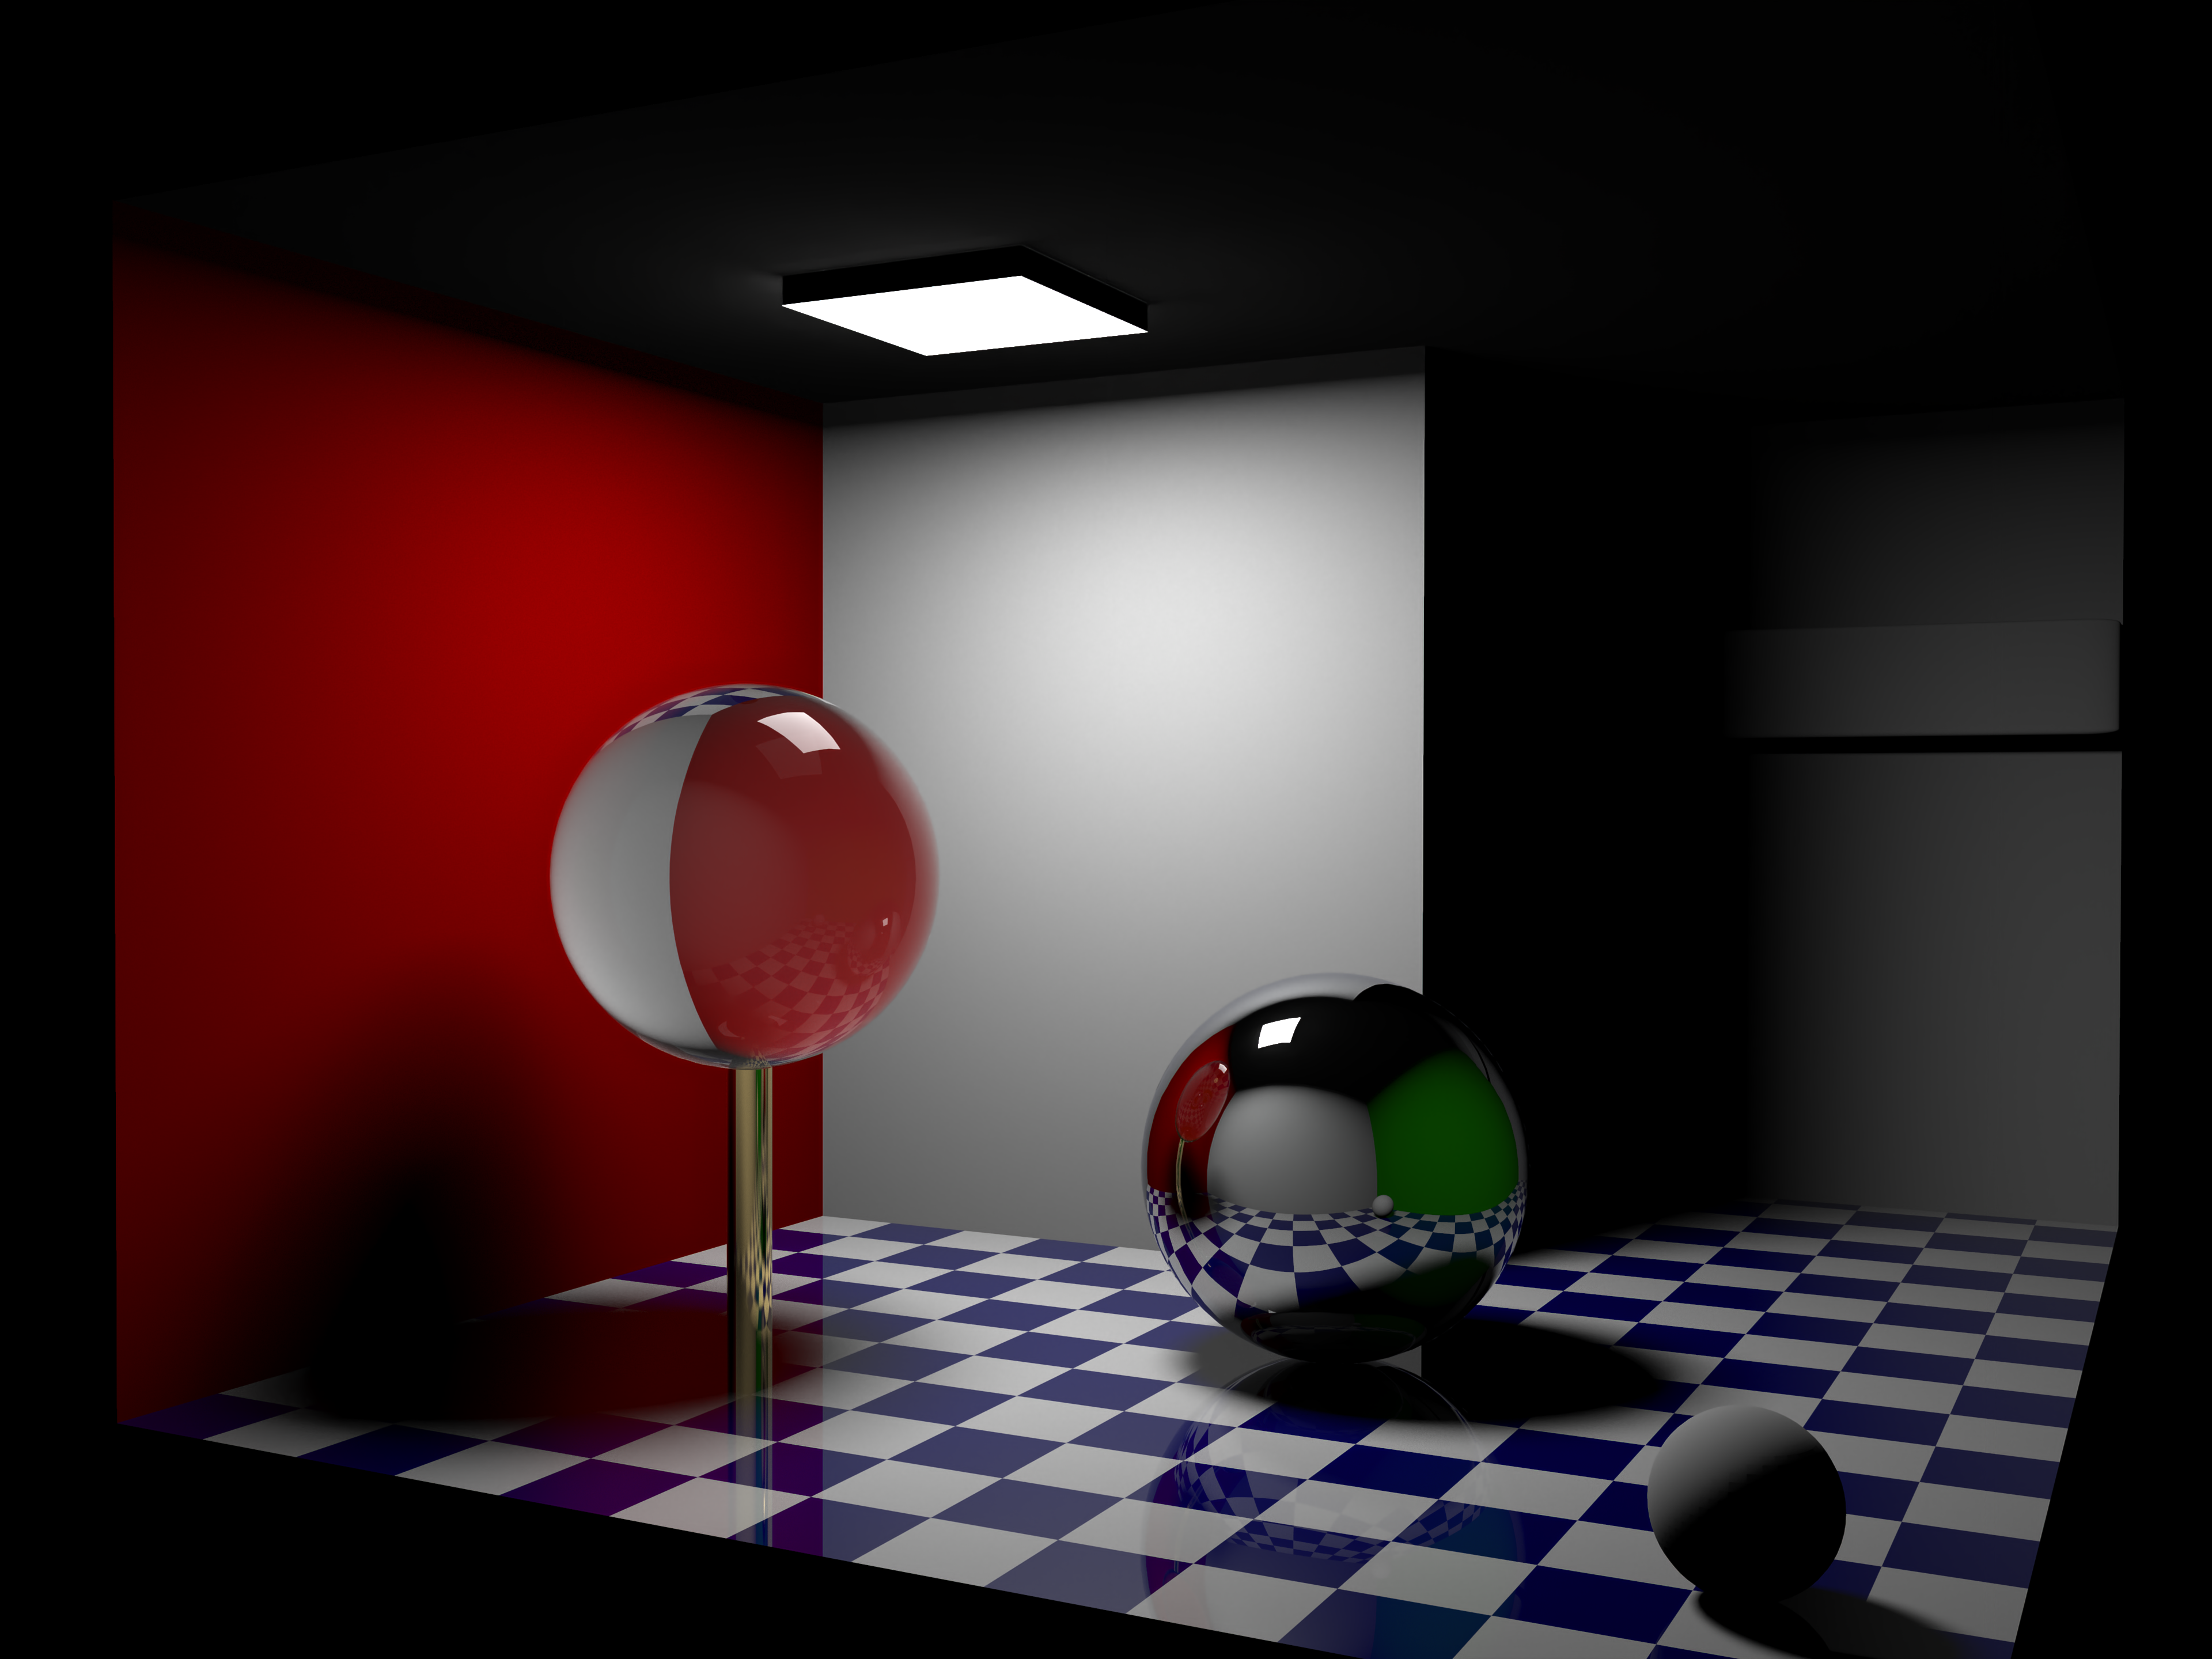
\includegraphics[scale=0.65]{Graphics/Direct_lighting.png}
		\caption{Scene lighting with direct illumination only. By Barahag - Own work, CC BY-SA 4.0}
		\url{https://commons.wikimedia.org/w/index.php?curid=88541991}
		\label{gra:Direct Illumination}
	\end{minipage}\hfill
	\begin{minipage}{0.48\textwidth}
		\centering
		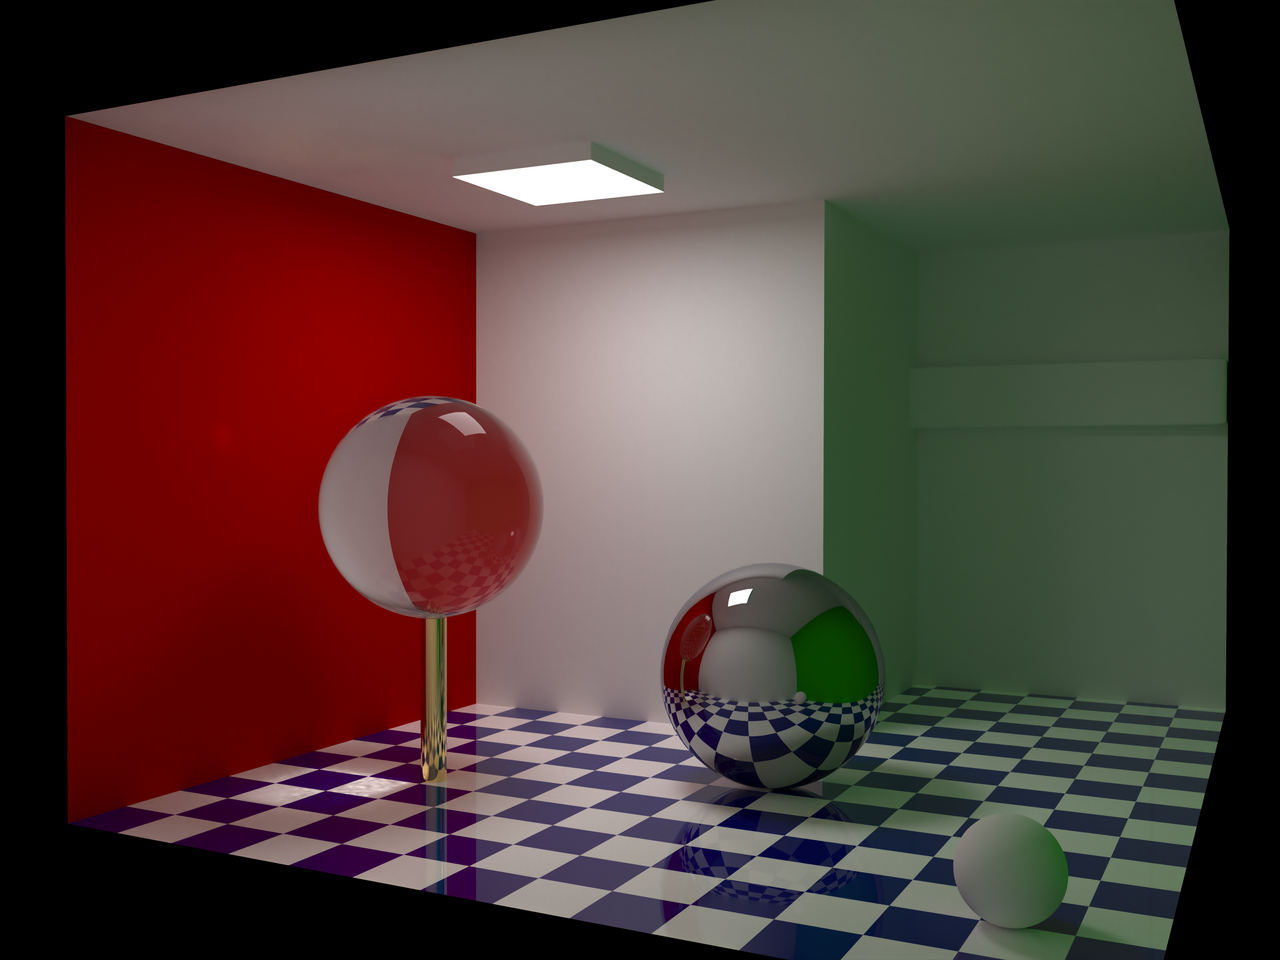
\includegraphics[scale=0.65]{Graphics/Global_illumination.png}
		\caption{Scene lighting with Global illumination. By Barahag - Own work, CC BY-SA 4.0}
		\url{https://commons.wikimedia.org/w/index.php?curid=88540888}
		\label{gra:Global Illumination}
	\end{minipage}
\end{figure}

The field-standard for accurate lighting and shadows in a scene is Path-Tracing, a method that tracks every light ray and any interactions it has with the objects of a 3D scene and calculates the resulting color for each pixel of the screen. Such approach remains prohibitively expensive for most interactive applications, so real-time systems employ precomputation and approximation of the illumination of the scene; static geometry is baked into lightmaps that store per-texel irradiance, while dynamic elements sample from irradiance volumes or light probes, sparse 3D points whose spherical-harmonic coefficients are interpolated at runtime. 

Screen-space GI methods typically approximate a limited number of light-ray bounces directly from the camera's depth buffer, but suffer from missing contextual information outside the camera's view frustum and temporal instability. Voxel-based approaches (e.g., cone-tracing through a low resolution 3D grid) % citation?
enable more dynamic multi-bounce effects at the cost of memory, processing cost and potential blurring of fine detail. 

Across all these techniques, the central challenge is allocating a strict millisecond-scale budget to indirect illumination while maintaining consistency across static and dynamic scene content, avoiding visible seams when blending baked and runtime solutions and fitting within GPU memory constraints. 

Light probes, in particular, represent a compelling middle-ground, flexible enough to illuminate moving objects without rebaking yet compact enough for real-time evaluation, making their optimal placement a critical factor in any high-quality GI pipeline.

% citations where needed?
% fix typos if any, better wording at 1 and 2 paragraph?

%\pagebreak % temporary potentially	

\section{Related Work}
There is an abundance of work in the literature addressing the problem of Global Illumination. These studies aim to achieve realistic lighting in 3D scenes by employing various approaches and techniques, each offering unique advantages and disadvantages, but they share a common goal: to maximize visual fidelity while minimizing computational costs.

\subsection{Offline Methods}
\label{sec:offline}
Offline Illumination methods refer to techniques that are not viable for real-time applications and are therefore used only in situations where the importance of high visual fidelity far outweighs the need for computational speed, typically in non-interactive 3D renders, most commonly in movies or pre-rendered scenes. Classic Path-Tracing, first introduced in 1986 \parencite{Kajiya1986}, tracks the movement of a photon ray emitted from a source, typically the camera, and simulates physics interactions to calculate the color of each screen pixel accurately. The immense computational cost of path-tracing led to the development of performance improvements, such as the Metropolis Light Transport (MLT) method introduced in 1997 \parencite{Veach1997}, and variants like bi-directional Path-Trace \parencite{Lafortune1993}, which build on Monte-Carlo algorithms \parencite{Lafortune1996}.

\subsection{Online Methods} % maybe section these?
In contrast, online methods aim to calculate GI interactions in real-time, most commonly used in interactive applications like video games or simulations. They try to balance performance and accuracy, a task that is often difficult due to the processing cost of the calculations for a realistic result. Therefore, these methods take shortcuts, either approximating the GI interactions to a certain degree to maintain framerate budgets, or by precomputing some of the data, wherever possible.

\subsection*{Traditional Methods} % rename this to something better
Techniques that precompute the illumination of a scene only do so for static geometry; objects in the scene that will never change their position, rotation or scale. The algorithms "bake" the required information onto texture maps, which are rendered as such when needed. Light-mapping is one such technique. It precomputes surface brightness and has a low runtime cost. The game Quake was the first interactive application that used lightmaps for rendering GI \parencite{WikiLightmaps}.

Another early technique is the Irradiance Volumes algorithm  \parencite{Greger1998}, which scatters spherical-harmonic (SH) irradiance samples on a 3D grid on the scene. At runtime, lighting is interpolated from the nearest SH cells; this underlies many probe systems, like Unity's light-probe system that implicitly implements a sparse irradiance volume.

More recent static-GI algorithms include Light Field Probes \parencite{McGuire2017}. Light Field Probes extend standard irradiance probes by additionally storing per-texel visibility for each probe. Furthermore, \parencite{Xu2022} introduce Discrete Visibility Fields for static ray-traced lighting. The method precomputes occlusion masks stored in a uniform voxel grid, and at runtime, rays that hit a cell use the stored precomputed masks to quickly cull visibility, skipping geometry already known to be occluded.

Unity's new Adaptive Probe Volumes (APV) build on irradiance volumes by automatically populating a grid, with density matched to local geometry. APV then performs per-pixel probe sampling; each pixel blends from the eight nearest probes \parencite{Unity2025}.

Additionally, there are methods that don't focus on Probes for GI. A prevalent example is Unreal Engine's Lumen, a dynamic GI and reflections system that uses a hybrid tracing approach; It starts with a cheap screen-space or signed-distance-field ray cast, and then falls back to more expensive methods like hardware ray tracing \parencite{Unreal2025}.

NVIDIA has also developed RTXGI, a GPU-accelerated library implementing Dynamic Diffuse GI, using a volumetric grid of irradiance probes, which update every frame using hardware-accelerated ray tracing, creating accurate results at the cost of hardware-restricted algorithms and a relatively escalated cost of calculation \parencite{Nvidia2024}.

In 2011 \parencite{Crassin2011} , a Voxel Cone Tracing (VCT) technique was introduced to approximate real-time GI. In VCT, the scene's static geometry and lighting are "voxelized" into a 3D texture with multiple levels of mipmapping, containing radiance and opacity. At runtime, indirect illumination is approximated by tracing a few low-resolution "cones" from each surface sample into the aforementioned voxel grid, summing the values from regions of voxels.\newline

Even though there are numerous methods trying to solve real-time GI issues, a big percentage of them tend to revolve around probes of various types; most commonly calculating irradiance values among other high-importance metrics. Therefore, it is vital for a 3D scene to have proper probe placement for best results. There are a few methods that try to automate that process, often by placing the probes in a regular grid and only removing the probes that are inside objects, but that can lead to over-sampling, leading to performance costs, mainly in memory usage budgets. Furthermore, some techniques try to remove additional probes using heuristic methods, therefore approaching optimal placement, but with a significant precomputational cost.

In \parencite{Wang2019}, an automatic non-uniform placing scheme  is introduced, which uses 3D scene skeletons and gradient-descent refinement to cover important locations without redundant probes. A very recent work formulates geometry-based optimization of probe placement using various mesh features, to further improve the lighting in VR/AR scenarios \parencite{Teuber2024}.

Similarly, \parencite{Vardis2021} approach the problem by starting with a probe set on a dense grid and iteratively removing the least-important probes using radiance error tests, preserving the global light field while minimizing probe count.

\subsection*{AI-based Methods}
Recently, AI-assisted methods have started to be developed in order to improve GI in 3D applications, specifically in probe-based solutions. In \parencite{Guo2022}, they propose a hybrid neural probe GI. They use a gradient-based search to re-project stored probe radiance for any view, therefore eliminating parallax, and then apply a small neural network to reconstruct high-quality images from low-resolution probe data. Related, a Neural Light Field Probes method has been introduced \parencite{You2024}, which works by decomposing a scene into a grid of trainable light field probes. Each of these probes encodes local radiance and visibility in a compact feature map. Finally, a neural network optimizes these probes so that the summation of their contributions reproduces the full scene lighting. 

\section{Thesis Structure} % redo parts of this, fix stuff
The structure of the remainder of this thesis will be described shortly. Chapter \ref{sec:Background}, titled Background, covers important information about light probes and their implementation, describes the AI model basis that was used for our implementation, and introduces the tools and technologies that were used in this thesis. Chapter \ref{sec:Approach}, titled Our Approach, presents our method, describes the implementation of the algorithms used, and explains how each part is combined to create the Light-Probe Neural Network (LPNN), our neural network system that attempts to speed up light probe placement in Unity 3D scenes by predicting importance values for the given grid set and placing only the most vital light probes, affected by a user-controlled threshold value. Each grid position gathers samples of a few metrics, which are then used by the neural network to decide whether or not it is vital to place a light probe in each individual cell of the 3D grid. A step-by-step process of creating the grid, getting the features out of the grid cells, and placing the probes and baking the global illumination inside Unity. Additionally, the feature set can be used to retrain the AI model, we explain how to create the labels needed for the process, and how to import the new model to Unity using Sentis for usage. Chapter \ref{sec:Experiments}, titled Experiments, presents an experimental comparative and qualitative evaluation between the proposed method and some of the already introduced algorithms. Finally, Chapter \ref{sec:Conclusions}, titled Conclusions and Future Works, concludes the thesis and proposes directions for future work based on this thesis.












